%\documentclass[makeidx,envcountchap,graybox,deutsch,ngerman,sectrefs]{svmono}
%\documentclass[envcountchap,graybox,deutsch,sectrefs]{svmono}
%%%%% eigene tempor�re Abk�rzungsliste, f�r die Zeit, bis einheitliche Schreibungen bestehen
\usepackage{tempshort}
%%  Von Springer empfohlene Pakete %% 
%%\documentclass[envcountsect,graybox,deutsch,sectrefs]{svmono}
\usepackage{chapterbib}
\usepackage{type1cm}
\usepackage[ansinew]{inputenc}
\usepackage{babel}
\usepackage[pdftex]{graphicx} %PDF-Vektorgrafiken einbinden
\usepackage{newtxtext} %Typischer Springer-Font
\usepackage{newtxmath}
\usepackage{multicol}
\usepackage[bottom]{footmisc} %Platziert alle Fu�noten unten  
\usepackage[nobreak]{cite}
%\usepackage{biblatex}
\usepackage{cancel}
\usepackage[absolute]{textpos}
\usepackage{graphicx}
\usepackage{pdfpages}

%\usepackage{floatrow}
%\usepackage{mwe}
\usepackage[figuresright]{rotating}
\usepackage{bigints}
\let\laplace\relax  % Vermeidung der Fehlermeldung "\laplace already defined."
\usepackage{trfsigns}
\usepackage{amsmath}
\usepackage{tabulary}
\usepackage{tabularx}

%%  Eigene Pakete %%
\usepackage{adjustbox}
\usepackage{wasysym}
\usepackage{gensymb}
\usepackage{float}
\usepackage{caption}
\usepackage[left=5cm,right=4cm,top=3cm,bottom=4cm,includeheadfoot]{geometry}

%\usepackage{wasysym}
%\usepackage{bigints}
%\usepackage{esint}
%\usepackage{relsize,exscale}

\usepackage{mathtools}   % Vermeidung der Fehlermeldung "Undefined control sequence \coloneqq."


% header and footer
\usepackage{fancyhdr}
\pagestyle{fancy}
\fancyhead[LE,RO]\thepage
\renewcommand{\sectionmark}[1]{\markright{\thesection.\ #1}}
%\fancyhead[LO]{\nouppercase\leftmark}
%\fancyhead[RE]{\nouppercase\rightmark}
\fancyhead[LO]{\nouppercase\rightmark}
\fancyhead[RE]{\nouppercase\leftmark}
\fancyfoot{}
% svmono hat offenbar irgendwas merkw�rdig definiert, darum mu� hier verbreitert werden
%\addtolength\headwidth{25pt}
\setlength{\headheight}{25pt}

%% Units
\usepackage{siunitx}
\sisetup{
  locale = US,
  per-mode = reciprocal, %symbol, % | reciprocal | fraction | ?
  exponent-product = \cdot,
  separate-uncertainty,
  %exponent-to-prefix,
  %prefixes-as-symbols = false,
  %list-units = brackets,% | single | repeat
  %range-units = brackets,% | single | repeat
  %multi-part-units = brackets,% | single | repeat
}
\usepackage{chngcntr}
\usepackage{booktabs}
\usepackage{slashed}
\usepackage{listings}
\usepackage{color} %red, green, blue, yellow, cyan, magenta, black, white
%\usepackage{color} %Einfache Farbendefinition -> von Graybox-Option ben�tigt
\usepackage{multirow}
\usepackage{longtable} %Tabellen �ber mehrere Seiten hinweg
\usepackage{framed} % von Graybox-Option ben�tigt
\usepackage[shortlabels]{enumitem} %Erweiterte Aufz�hloptionen
\usepackage{array}
\usepackage[xindy]{imakeidx} %Wortindex und Personenindex erstellen

\usepackage[hyphens]{url}
%\usepackage[breaklinks,colorlinks=true,linkcolor=black,urlcolor=blue,citecolor=black,filecolor=green,hyperfootnotes=false]{hyperref}
\usepackage[                                    %Hyperref erstellt ein Bookmark/Lesezeichen im PDF. siehe https://www.namsu.de/Extra/pakete/Hyperref.html
bookmarksopen=true,															%Das Lesezeichen ist ge�ffnet beim �ffnen der PDF.
bookmarksnumbered=true,                         %Zahlen werden im Bookmark angezeigt.   
plainpages=false,
pdfpagelabels,
colorlinks=true,                                %Links werden farbig dargestellt.
linkcolor=black, citecolor=black, urlcolor=cyan %Farben definieren.
]{hyperref}                                     %Sollte als letztes eingebunden werden, da es sehr viele Verweise und �nderungen erzeugt. Das Packet ist sehr stark, aber auch umfangreich ist. 

%\usepackage[breaklinks,colorlinks=true,linkcolor=black,urlcolor=blue,citecolor=black,filecolor=green,hyperfootnotes=false]{hyperref}
%\usepackage[breaklinks,colorlinks=true,linkcolor=black,urlcolor=blue,citecolor=black,filecolor=green,hyperfootnotes=false
            %pdftex,
            %pdfauthor={Kaschke, Cartarius},
            %pdftitle={Finger�bungen der Physik}
            %pdfsubject={Ein Repetitorium und �bungsbuch zu im Studium wenig behandelten Kapiteln der Physik mit ausf�hrlich behandelten Problemen und MATLAB-Programmen},
            %pdfkeywords={Physik, Mechanik}
            %]{hyperref}
\pdfminorversion=5

\usepackage{hypcap}
\usepackage[record,section=section,stylemods={mcols},automake]{glossaries-extra}
\usepackage{glossary-longextra}
%\usepackage{glossary-bookindex}
%\makeindex
\setglossarystyle{long-name-sym-desc-loc}
\setabbreviationstyle[acronym]{long-short}

\definecolor{killA}{rgb}{.7,.3,.3}
\newcommand\killA[1]{\bgroup\color{killA}{\cancel{#1}}\egroup}
\newcommand\killB[1]{\bgroup\color{cyan!30!black}{\cancel{#1}}\egroup}

% typographisch korrekte Abk�rzungen (needs to be loaded after hyperref)
\usepackage{abbrev}
\newglossary*{bew}{Glossar}
\newglossary*{hm}{Glossar}
\newglossary*{adyn}{Glossar}
\newglossary*{kontmech}{Glossar}
\newglossary*{aero}{Glossar}
\newglossary*{edyn}{Glossar}
\newglossary*{spo}{Glossar}
\newglossary*{optbas}{Glossar}
\newglossary*{optger}{Glossar}
\newglossary*{optatm}{Glossar}
\newglossary*{optspez}{Glossar}
\GlsXtrLoadResources[src={bew/gloss},type=bew]
\GlsXtrLoadResources[src={hm/gloss},type=hm]
\GlsXtrLoadResources[src={adyn/gloss},type=adyn]
\GlsXtrLoadResources[src={kontmech/gloss},type=kontmech]
\GlsXtrLoadResources[src={aero/gloss},type=aero]
\GlsXtrLoadResources[src={spo/gloss},type=spo]
\GlsXtrLoadResources[src={edyn/gloss},type=edyn]
\GlsXtrLoadResources[src={optbas/gloss},type=optbas]
\GlsXtrLoadResources[src={optger/gloss},type=optger]
\GlsXtrLoadResources[src={optatm/gloss},type=optatm]
\GlsXtrLoadResources[src={optspez/gloss},type=optspez]
\glssetcategoryattribute{bew}{indexname}{true}
%\renewcommand\index\newterm
%\newcolumntype{g}[1]{>{\RaggedRight\hspace{0pt}}p{#1}}
%\renewcommand\glslongextraNameAlign{g}
\renewcommand\glslongextraLocationAlign{@{\ ~\ }>{\raggedright}p{\glspagelistwidth}}
\definecolor{gls}{rgb}{.4,.4,.5}
\renewcommand*{\glstextformat}[1]{\textcolor{gls}{#1}}

%Absatzregeln
\clubpenalty = 30000 %Keine einzelnen Absatzzeilen
\widowpenalty = 30000
\setlength{\parindent}{0em} 
\newcolumntype{L}[1]{>{\raggedright\arraybackslash}p{#1}}
\newcolumntype{C}[1]{>{\centering\arraybackslash}p{#1}}
\newcolumntype{R}[1]{>{\raggedleft\arraybackslash}p{#1}}

\usepackage{xstring}

\newcommand\mfile[2]{%
\saveexpandmode\noexpandarg
\StrSubstitute{#2}{_}{\_}[\tmpname]
\restoreexpandmode
\href{MatlabDateien/\chapname/#1\tmpname}{\tmpname}}

%%% Hyperlinks zu MATLAB Dateien
%\newcommand\mlref[1]{\mfile{}{#1}}
%\newcommand\mlinclref[1]{\mfile{IncludeFolder/}{#1}}
%\newcommand\mldataref[1]{\mfile{Data/}{#1}}

%%% .. f�r ein Verzeichnis hoch
%%% . f�r aktuelle Verzeichnis
%% lokal: MatlabDateien/bew
%\newcommand\mlbewref[1]{\href{MatlabDateien/bew/#1}{#1}}
%% git: https://github.com/sn-code-inside/fingeruebungen-physik/tree/main/bew

\newcommand{\mlrefwithindex}[2]{%
  \index[mfiles]{#2}%   <-- Eintrag im M-File-Index mit aktueller Seitenzahl
  \href{https://github.com/sn-code-inside/fingeruebungen-physik/tree/main/#1/#2}{#2}%
}


%\newcommand\mlbewref[1]{\href{https://github.com/sn-code-inside/fingeruebungen-physik/tree/main/bew/#1}{#1}}
%\newcommand\mlbewdref[1]{\href{https://github.com/sn-code-inside/fingeruebungen-physik/tree/main/bew/Data/#1}{#1}}
%\newcommand\mlbewiref[1]{\href{https://github.com/sn-code-inside/fingeruebungen-physik/tree/main/bew/IncludeFolder/#1}{#1}}
%\newcommand\mlkontmechref[1]{\href{https://github.com/sn-code-inside/fingeruebungen-physik/tree/main/kontmech/#1}{#1}}
%\newcommand\mlkontmechdref[1]{\href{https://github.com/sn-code-inside/fingeruebungen-physik/tree/main/kontmech/Data/#1}{#1}}
%\newcommand\mlkontmechiref[1]{\href{https://github.com/sn-code-inside/fingeruebungen-physik/tree/main/kontmech/IncludeFolder/#1}{#1}}
%\newcommand\mlhmref[1]{\href{https://github.com/sn-code-inside/fingeruebungen-physik/tree/main/hm/#1}{#1}}
%\newcommand\mlhmdref[1]{\href{https://github.com/sn-code-inside/fingeruebungen-physik/tree/main/hm/Data/#1}{#1}}
%\newcommand\mlhmiref[1]{\href{https://github.com/sn-code-inside/fingeruebungen-physik/tree/main/hm/IncludeFolder/#1}{#1}}
%\newcommand\mladynref[1]{\href{https://github.com/sn-code-inside/fingeruebungen-physik/tree/main/adyn/#1}{#1}}
%\newcommand\mladyndref[1]{\href{https://github.com/sn-code-inside/fingeruebungen-physik/tree/main/adyn/Data/#1}{#1}}
%\newcommand\mladyniref[1]{\href{https://github.com/sn-code-inside/fingeruebungen-physik/tree/main/adyn/IncludeFolder/#1}{#1}}
%\newcommand\mledynref[1]{\href{https://github.com/sn-code-inside/fingeruebungen-physik/tree/main/edyn/#1}{#1}}
%\newcommand\mledyndref[1]{\href{https://github.com/sn-code-inside/fingeruebungen-physik/tree/main/edyn/Data/#1}{#1}}
%\newcommand\mledyniref[1]{\href{https://github.com/sn-code-inside/fingeruebungen-physik/tree/main/edyn/IncludeFolder/#1}{#1}}
%\newcommand\mloptbasref[1]{\href{https://github.com/sn-code-inside/fingeruebungen-physik/tree/main/optbas/#1}{#1}}
%\newcommand\mloptbasdref[1]{\href{https://github.com/sn-code-inside/fingeruebungen-physik/tree/main/optbas/Data/#1}{#1}}
%\newcommand\mloptbasiref[1]{\href{https://github.com/sn-code-inside/fingeruebungen-physik/tree/main/optbas/IncludeFolder/#1}{#1}}
%\newcommand\mloptspezref[1]{\href{https://github.com/sn-code-inside/fingeruebungen-physik/tree/main/optspez/#1}{#1}}
%\newcommand\mloptspezdref[1]{\href{https://github.com/sn-code-inside/fingeruebungen-physik/tree/main/optspez/Data/#1}{#1}}
%\newcommand\mloptspeziref[1]{\href{https://github.com/sn-code-inside/fingeruebungen-physik/tree/main/optspez/IncludeFolder/#1}{#1}}

\newcommand\mlbewref[1]{\mlrefwithindex{bew}{#1}}
\newcommand\mlbewdref[1]{\mlrefwithindex{bew/Data}{#1}}
\newcommand\mlbewiref[1]{\mlrefwithindex{bew/Include}{#1}}
\newcommand\mlkontmechref[1]{\mlrefwithindex{kontmech}{#1}}
\newcommand\mlkontmechdref[1]{\mlrefwithindex{kontmech/Data}{#1}}
\newcommand\mlkontmechiref[1]{\mlrefwithindex{kontmech/Include}{#1}}
\newcommand\mlhmref[1]{\mlrefwithindex{hm}{#1}}
\newcommand\mlhmdref[1]{\mlrefwithindex{hm/Data}{#1}}
\newcommand\mlhmiref[1]{\mlrefwithindex{hm/Include}{#1}}
\newcommand\mladynref[1]{\mlrefwithindex{adyn}{#1}}
\newcommand\mladyndref[1]{\mlrefwithindex{adyn/Data}{#1}}
\newcommand\mladyniref[1]{\mlrefwithindex{adyn/Index}{#1}}
\newcommand\mledynref[1]{\mlrefwithindex{edyn}{#1}}
\newcommand\mledyndref[1]{\mlrefwithindex{edyn/Data}{#1}}
\newcommand\mledyniref[1]{\mlrefwithindex{edyn/Index}{#1}}
\newcommand\mloptbasref[1]{\mlrefwithindex{optbas}{#1}}
\newcommand\mloptbasdref[1]{\mlrefwithindex{optbas/Data}{#1}}
\newcommand\mloptbasiref[1]{\mlrefwithindex{optbas/Include}{#1}}
\newcommand\mloptspezref[1]{\mlrefwithindex{optspez}{#1}}
\newcommand\mloptspezdref[1]{\mlrefwithindex{optspez/Data}{#1}}
\newcommand\mloptspeziref[1]{\mlrefwithindex{optspez/Include}{#1}}
\newcommand\mloptgerref[1]{\mlrefwithindex{optger}{#1}}
\newcommand\mloptgerdref[1]{\mlrefwithindex{optger/Data}{#1}}
\newcommand\mloptgeriref[1]{\mlrefwithindex{optger/Include}{#1}}
\newcommand\mloptatmref[1]{\mlrefwithindex{optatm}{#1}}
\newcommand\mloptatmdref[1]{\mlrefwithindex{optatm/Data}{#1}}
\newcommand\mloptatmiref[1]{\mlrefwithindex{optatm/Include}{#1}}



\newcommand\mlcmd[1]{\textcolor{cyan}{\texttt{#1}}}

%Grafikregeln
\graphicspath{{hm/graphs/}
	                    	{bew/graphs/}
     						{kontmech/graphs/}
							{hm/graphs/}
							{adyn/graphs/}
							{edyn/graphs/}
							{kontmech/graphs/}
							{spo/graphs/}
							{optbas/graphs/}
							{optger/graphs/}
							{optatm/graphs/}
							{solman/graphs/}
                                                        {aero/graphs}}
\DeclareGraphicsExtensions{.pdf, .png, .jpg, .jpeg}
\def\figname{Abb}
\newcommand\figref[1]{\figname.\ \ref{abb:#1}}
\usepackage[labelfont=bf]{caption}

\usepackage{tocloft}
\usepackage{etoc}
\setlength\cftfignumwidth{30pt}

% Flatterrand links
\cftsetindents{chapter}{0em}{4em}
\cftsetindents{section}{1.5em}{4em}
\cftsetindents{subsection}{3.8em}{4em}

% flacher Rand links
%\cftsetindents{chapter}{0em}{4em}
%\cftsetindents{section}{0em}{4em}
%\cftsetindents{subsection}{0em}{4em}

\newcommand\partitle[1]{
\addcontentsline{toc}{part}{#1}
\begin{titlepage}
  %\vskip 60%\p@
  \begin{center}
    {\LARGE Finger�bungen der Physik -- #1 \par}
    \vskip 3em%
    {\large Michael Kaschke und Holger Cartarius\par}
  \end{center}
\end{titlepage}
}

%\newcommand\mlref[1]{\href{\chapname/matlab/#1}{#1}}
%\newcommand\mlinclref[1]{\href{\chapname/matlab/IncludeFolder/#1}{\color{cyan}{#1}}}

%Neue Kommandos
\newcommand{\lk}{\left(}        %gro�e runde Klammer (links)
\newcommand{\rk}{\right )}      %gro�e runde Klammer (rechts)
\newcommand{\lgk}{\left \{}     %gro�e geschweifte Klammer (links)
\newcommand{\rgk}{\right \}}    %gro�e geschweifte Klammer (rechts)
\newcommand{\lek}{\left [}      %gro�e eckige Klammer (links)
\newcommand{\rek}{\right ]}     %gro�e eckige Klammer (rechts)
\newcommand{\anf}[1]{\glqq#1\grqq}    %Deutsche Anf�hrungszeichen: \anf{}
\newcommand{\defined}{:=}				%Definition
\newcommand{\curl}{\text{\textbf{rot}}\,}	%Rotation-Operator curl()
\newcommand{\ket}[1]{|#1\rangle}		%Quantenmechanischer Zustand
\newcommand{\curvelintri}{\,\overset{\blacktriangle}{\smallfrown}}
\newcommand{\straighttri}{\blacktriangle}
\newcommand{\UT}{\text{UT}}
\newcommand{\UTC}{\text{UTC}}
\newcommand{\JD}{\text{JD}}
\newcommand{\JDE}{\text{JDE}}
\newcommand{\MJD}{\text{MJD}}
\newcommand{\TDT}{\text{TDT}}
\newcommand{\TT}{\text{TT}}
\newcommand{\NVS}{\text{Navier-Stokes-Gleichungen}}
\newcommand{\MWG}{\text{Maxwell-Gleichungen}}
\newcommand{\EMW}{\text{Elektromagnetische Wellen}}
\newcommand{\eMW}{\text{elektromagnetischen Wellen}}
\newcommand{\RT}{\text{Relativit�tstheorie~}}
\newcommand{\au}{\mathrm{AE}}
\newcommand{\ET}{\text{ET}}
\newcommand{\TAI}{\text{TAI}}
\newcommand{\GMST}{\text{GMST}}
\newcommand{\LMST}{\text{LMST}}
\newcommand{\MESZ}{\text{MESZ}}
\newcommand{\KOS}{\text{Koordinatensystem }}
\newcommand{\DGL}{\text{Differentialgleichung }}
\newcommand{\NA}{\text{NA}}
\newcommand{\uA}{\text{u}}  %atomare Masseneinheit
\newcommand{\MOZ}{\text{MOZ}}
\newcommand{\grad}{\text{\textbf{grad}}\,}	%Gradient-Operator grad()
\newcommand{\uproman}[1]{\mathrm{\uppercase\expandafter{\romannumeral#1}}}
\newcommand{\lowroman}[1]{\romannumeral#1\relax}

\newcommand\todo[1]{\textcolor{red}{TODO: #1}}

\renewcommand{\=}[1]{\stackrel{\text{#1}}{=}}  %Schrift �ber Gleich-Zeichen
\renewcommand{\d}{\partial}
\newcommand{\lra}{\Leftrightarrow}  %�quivalenz-Pfeile
\newcommand{\abs}[1]{\left\vert#1\right\vert}     %Betragsklammern
\renewcommand{\Re}{\mathrm{Re}}                          %Realteil
\renewcommand{\Im}{\mathrm{Im}}                          %Imagin�rteil
\renewcommand{\im}{\mathrm{i}}                         %Imagin�re Einheit
\renewcommand{\epsilon}{\varepsilon} 
\newcommand{\keff}{k_\text{eff}}
\newcommand{\con}{\text{const}}
\newcommand{\conv}{\vec{const}}
\newcommand{\PL}{\mathcal{P}_}
\newcommand{\artanh}{\mathrm{artanh}}
% QED-Symbol im text- bzw. Mathemodus
\newcommand{\textqed}{\hfill ~ $\square$}
\newcommand{\mmqed}{\tag*{$\square$}}

\newcommand{\fa}{(\textbf{a}) }
\newcommand{\fb}{(\textbf{b}) }
\newcommand{\fc}{(\textbf{c}) }
\newcommand{\fd}{(\textbf{d}) }
\newcommand{\fe}{(\textbf{e}) }
\newcommand{\ff}{(\textbf{f}) }

\newcommand{\iF}{im Folgenden~}
\newcommand{\iA}{im Allgemeinen~}


\DeclareMathOperator\divv{div}
\DeclareMathOperator\res{Res}
\DeclareMathOperator{\sech}{sech}
\DeclareMathOperator\sgn{sgn}

% f�r Appendix - MATLAB Referenz
\newcommand{\rotv}{\vec{rot}\,}
\newcommand{\gradv}{\vec{grad}\,}
\newcommand{\nablav}{\vec{\nabla}\,}

\newcommand{\ceil}{\mathrm{ceil}}
\newcommand{\sinc}{\mathrm{sinc}}
\newcommand{\diag}{\mathrm{diag}}
\newcommand{\sign}{\mathrm{sign}}
\newcommand{\length}{\mathrm{length}}
\newcommand{\sort}{\mathrm{sort}}
\newcommand{\summ}{\mathrm{sum}}
\newcommand{\asin}{\mathrm{asin}}
\newcommand{\acos}{\mathrm{acos}}
\newcommand{\atan}{\mathrm{atan}}
\newcommand{\prodd}{\mathrm{prod}}
\newcommand{\median}{\mathrm{mediab}}
\newcommand{\mean}{\mathrm{mean}}
\newcommand{\std}{\mathrm{std}}
\newcommand{\eye}{\mathrm{eye}}
\newcommand{\zeros}{\mathrm{zeros}}
\newcommand{\ones}{\mathrm{ones}}
\newcommand{\rand}{\mathrm{rand}}
\newcommand{\inline}{\mathrm{inline}}
\newcommand{\modd}{\mathrm{mod}}
\newcommand{\floor}{\mathrm{floor}}
\newcommand{\round}{\mathrm{round}}
\newcommand{\rem}{\mathrm{rem}}
\newcommand{\sqrtt}{\mathrm{sqrt}}
\newcommand{\triu}{\mathrm{triu}}
\newcommand{\tril}{\mathrm{tril}}
\newcommand{\size}{\mathrm{size}}
\newcommand{\dett}{\mathrm{det}}
\newcommand{\inv}{\mathrm{inv}}
\newcommand{\rank}{\mathrm{rank}}
\newcommand{\rref}{\mathrm{rref}}
\newcommand{\eig}{\mathrm{eig}}
\newcommand{\poly}{\mathrm{poly}}
\newcommand{\lu}{\mathrm{lu}}
\newcommand{\qr}{\mathrm{qr}}
\newcommand{\quaddd}{\mathrm{quad}}
\newcommand{\fzero}{\mathrm{fzero}}
\newcommand{\roots}{\mathrm{roots}}
\newcommand{\odezd}{\textcolor{mygreen}{\texttt{ode23}}}
\newcommand{\odevf}{\textcolor{mygreen}{\texttt{ode45}}}
\newcommand{\odeeds}{\textcolor{mygreen}{\texttt{ode13s}}}
\newcommand{\odeefs}{\textcolor{mygreen}{\texttt{ode15s}}}
\newcommand{\ddezd}{\textcolor{mygreen}{\texttt{dde23}}}
\newcommand{\onlineZ}{online verf�gbaren Zusatzmaterialien{}}
\newcommand{\MKc}{\url{https://www.fingeruebungen-physik.de}{}}
\newcommand{\linklsg}{\href{https://www.fingeruebungen-physik.de}{\textcolor{blue} {$\rightarrow$ L�sungsteil.}}}
\newcommand{\githubSN}{\url{https://github.com/sn-code-inside/fingeruebungen-physik}{}\,\,}

\newcommand{\FT}{\mathcal{F}} %Fourier-Transformierte

% Aufz�hlung der L�sungen der Teilaufgaben
\newlist{subprobs}{enumerate}{1}
\setlist[subprobs]{
  label= \textbf{\textit{Teilaufgabe}} \textbf{\textit{\arabic*:}} \protect\thissubprob,
  ref=\arabic*, itemsep=\baselineskip, align=left}
\newcommand{\subprob}[1]{
  \def\thissubprob{\textbf{\textit{#1}}}\item ~\vspace{0.2\baselineskip} \newline}

\renewenvironment{example}[1]{
\refstepcounter{example}\par\medskip
\begin{shaded} 
\begin{samepage}
\noindent \textbf{\textit{Beispiel~\theexample: {#1}}}\\ 
\noindent{\color{black} \rule{\textwidth}{0.2 mm}}
\end{samepage}
}{\end{shaded}
\noindent{\color{black} \rule{\textwidth}{0.2 mm}}
} % or snugshade
\definecolor{shadecolor}{gray}{0.95}
\definecolor{mygreen}{RGB}{28,172,0} % color values Red, Green, Blue
\definecolor{mylilas}{RGB}{170,55,241}

\newenvironment{infobox}[1]{
     \begin{shaded} 
     \begin{samepage}
\noindent{\color{black} \rule{\textwidth}{0.2 mm}}
     \end{samepage}
}{\end{shaded}
\noindent{\color{black} \rule{\textwidth}{0.2 mm}}
} 
\definecolor{shadecolor}{gray}{0.95}
\definecolor{mygreen}{RGB}{28,172,0} % color values Red, Green, Blue
\definecolor{mylilas}{RGB}{170,55,241}


\newenvironment{nebenrechnung}[1]{
\begin{shaded} 
\begin{samepage}
\noindent\textbf{Nebenrechnung: \\} 
\noindent{\color{black} \rule{0.1\columnwidth}{0.2mm} \\}
\end{samepage}
}{\end{shaded}
\noindent{\color{black} \rule{0.1\columnwidth}{0.2mm} \\}
} % or snugshade
\definecolor{shadecolor}{gray}{0.95}
\definecolor{mygreen}{RGB}{28,172,0} % color values Red, Green, Blue
\definecolor{mylilas}{RGB}{170,55,241}

\newenvironment{merksatz}[1]{
\begin{shaded} 
\begin{samepage}
\noindent\textbf{Merke:\\} 
\noindent{\color{black} \rule{0.9\columnwidth}{0.2mm} \\ \\}
\end{samepage}
}{\end{shaded}
\noindent{\color{black} \rule{0.9\columnwidth}{0.2mm} \\}
} % or snugshade


\lstset{language=Matlab,%
    %basicstyle=\color{red},
    %basicstyle={\linespread{0.9}\ttfamily},
    basicstyle=\footnotesize\ttfamily,
    breaklines=true,%
    morekeywords={matlab2tikz},
    keywordstyle={\small \color{mygreen}},%
    morekeywords=[2]{1}, keywordstyle=[2]{\small\color{black}},
    identifierstyle={\small \color{black}},%
    stringstyle={\small\color{mylilas}},
    commentstyle={\small\color{mylilas}},%
    showstringspaces=false,%without this there will be a symbol in the places where there is a space
    numbers=left,%
    numberstyle={\tiny \color{black}},% size of the numbers
    numbersep=9pt, % this defines how far the numbers are from the text
    emph=[1]{for,end,else,break, function},emphstyle=[1]\small \color{blue}, %some words to emphasise
    emph=[2]{odeset},emphstyle=[2]\small \color{mygreen}, %some words to emphasise
    %emph=[2]{word1,word2}, emphstyle=[2]{style},    
}

%\bibliographystyle{spphys.bst}

%Trennregeln f�r spezielle Worte
%\hyphenation{Fresnel \matlab �qui-nok-ti-um}

\DeclareSIUnit\erg{erg}
\DeclareSIUnit\cal{cal}
\DeclareSIUnit\celsius{C}
\DeclareSIUnit\m{M}
\DeclareSIUnit\kel{K^{-4}}

%Stichwort- und Personenverzeichnis
\makeindex[title=Stichwortverzeichnis] % Create the default index
\makeindex[name=personen,title=Personenverzeichnis] % Create an index named 'personen'
\newcommand{\indexp}[1]{\index[personen]{#1}}
\makeindex[name=mfiles,title=MATLAB-Skriptverzeichnis,columns=2]

% list of exercises
\newcommand{\loxname}{\Large �bungsverzeichnis}  % einheitliche Gr��e Large
\newlistof[chapter]{prob}{lox}\loxname
\newcommand\uebung[3][]{\label{prob:#2}%
\addcontentsline{lox}{prob}{\protect\numberline{}{\probRef{#2}:~#3#1}}%
\textbf{#1#3}\\[\baselineskip]}
\makeatletter
\renewcommand{\l@prob}{\@dottedtocline{1}{0em}{0em}}
\makeatother

\newcommand\einfach{\uebung[~$\ast$~~]}
\newcommand\mittel{\uebung[~$\ast\,\ast$~~]}
\newcommand\schwierig{\uebung[~$\ast\,\ast\,\ast$~~]}
\newcommand\zusatz{\uebung[~$\ast\,\ast\,\ast\,!$~~]}
%\newcommand\einfach{\uebung[~\textbf{*}~~]}
%\newcommand\mittel{\uebung[~\textbf{*\,*}~~]}
%\newcommand\schwierig{\uebung[~\textbf{*\,*\,*}~]}
%\newcommand\zusatz{\uebung[~\textbf{*\,*\,*\,!}~~]}
\usepackage[atend]{bookmark}
%\BookmarkAtEnd{%
%\bookmarksetup{startatroot}\bookmark[level=0,named=\loxname]{}}

\newcommand\kapitel[1]{Kapitel \ref{kap:#1}}
%\newcommand\kap[1]{Kap.\ \ref{kap:#1}}
\newcommand\kap[1]{Kap. \ref{kap:#1}}

\begin{document}
% customize prob and sol in svmono
\makeatletter
%\counterwithin*{chapter}{part}

\spn@wtheorem{prob}{\bgroup\exercisename\egroup}{\bfseries}{\rmfamily}
\makeatother
\renewenvironment{sol}[1]{\par\addvspace{6pt}\noindent\phantomsection{\textbf{L�sung \ref{#1}}} \ignorespaces}{\par\addvspace{6pt}}
\newcommand\probRef[1]{�bung \ref{prob:#1}}
\renewcommand\probref[1]{\textbf{\probRef{#1}}}
\newcommand\lsgref[1]{L�sung \ref{lsg:#1}}

\newcommand\sbullet[1][.5]{\mathbin{\vcenter{\hbox{\scalebox{#1}{$\bullet$}}}}}

\setcounter{table}{0}



% f�r funktionierende Hyperlinks zwei neue Environments mit eigenen Countern, up. 2024-01-29
\newcounter{partsectionU}
\newcounter{partsectionL}
\newcounter{partsectionA}

\newenvironment{PartU}[1]
 {%
  \cleardoublepage
  \phantomsection
  \setcounter{section}{\value{partsectionU}}%
  \renewcommand{\thesection}{\"U\arabic{section}}%
  \renewcommand{\theHsection}{SU\arabic{section}}%
  \addcontentsline{toc}{part}{#1}%
  \thispagestyle{empty}
  \begin{flushright}
    \LARGE
    \textbf{
  �bungen\\ \bigskip  Band III\\ \bigskip Aerodynamik - Sportphysik\\}
  \end{flushright}
  \vspace*{\fill}
  \clearpage
 }
 {%
  \setcounter{partsectionU}{\value{section}}%
  \cleardoublepage
}

\newenvironment{PartL}[1]
 {%
  \cleardoublepage
  \phantomsection
  \setcounter{section}{\value{partsectionL}}%
  \renewcommand{\thesection}{L\arabic{section}}%
  \renewcommand{\theHsection}{SL\arabic{section}}%
  \addcontentsline{toc}{part}{#1}%
  \thispagestyle{empty}
  \begin{flushright}
    \LARGE
    \textbf{L�sungsvorschl�ge \\ \bigskip Band III \\ \bigskip Aerodynamik - Sportphysik\\}
  \end{flushright}
  \vspace*{\fill}
  \clearpage
 }
 {%
  \setcounter{partsectionL}{\value{section}}%
 \cleardoublepage
}

\newenvironment{PartA}[1]
 {%
  \cleardoublepage
  \phantomsection
  \setcounter{section}{\value{partsectionA}}%
  \renewcommand{\thesection}{A\arabic{section}}%
  \renewcommand{\theHsection}{SA\arabic{section}}%
  \addcontentsline{toc}{part}{#1}%
  \thispagestyle{empty}
  \begin{flushright}
    \LARGE
    \textbf{Appendix \\ \bigskip Band III \\ \bigskip Aerodynamik - Sportphysik\\}
  \end{flushright}
  \vspace*{\fill}
  \clearpage
 }
 {%
  \setcounter{partsectionA}{\value{section}}%
 \cleardoublepage
}


%%%%%%%%%%%%%%%%%%%%%%%%%%%%%%%%%%%%%%%%%%%%%%%%%%%%%%%%%%%%%

\bibliographystyle{spphys}

\makeatletter
\@addtoreset{chapter}{part}
\makeatother
\renewcommand{\thechapter}{�\,\arabic{chapter}}

\addtocontents{toc}{\protect\setcounter{tocdepth}{2}}% alles zeigen

\begin{PartU}{�bungen - Band III Aerodynamik - Sportphysik}
\setcounter{chapter}{3}
\setcounter{section}{2}
\setcounter{subsection}{0}
\setcounter{figure}{0}
\setcounter{equation}{0}
\setcounter{prob}{0}
\counterwithin{table}{section}
\setcounter{table}{0}
\newpage
\quad 
\thispagestyle{empty}
\newpage
\section{�bungsaufgaben}\label{kap:aero_uebungen}

\begin{prob} %�bung1
\einfach{aero_testpotential}{�berpr�fen auf die Existenz eines Potentials}

In Beispiel 2.4 wurde f�r die station�re Str�mung zwischen zwei W�nden
im Abstand $b$ das Geschwindigkeitsfeld
\begin{equation*}
  v_z(y) = \frac{1}{2\eta} \frac{\partial p(z)}{\partial z}
  \lk \lk y - \frac{b}{2} \rk^2 -  \frac{b^2}{4} \rk
\end{equation*}
gefunden. Analog ergab sich f�r ein Kreisrundes Rohr mit dem Durchmesser $R$
das Feld
\begin{equation*}
  v_z(r) = \frac{1}{4\eta} \frac{\partial p(z)}{\partial z}
  \lk r^2 - R^2 \rk \; .
\end{equation*}
�berpr�fen Sie beide Geschwindigkeitsfelder auf die Existens eines Potentials
und geben Sie dieses gegebenenfalls an.

\hyperref[lsg:aero_testpotential]{\textcolor{blue} {$\rightarrow$ L�sungsvorschlag}}\\
%\href{FingerUeb3_AB.pdf#lsg:aero_testpotential}{\textcolor{blue} {$\rightarrow$ L�sungsteil}}.\\

\noindent\rule[1ex]{\textwidth}{0.5pt}
\end{prob}

%%%%%%%%%%%%%%%%%%%%%%%%%%%%%%%%%%%%%%%%%%%%%%%%%%%%%%%%%%%%%%%%%%%%%%%%%%%%%


\begin{prob} %�bung2
\einfach{aero_potentialbeispiel}{Einfache Beispiele f�r Potentialstr�munen}

Stellen Sie die Potentialgleichungen f�r die Beispiele der Str�mung zwischen
zwei Platten und durch ein Kreisrundes Rohr aus \probref{aero_testpotential}
auf. �berzeugen Sie sich dabei am konkreten Beispiel, dass der Reibhungsterm
verschwindet. L�sen Sie die Potentialgleichung und berechnen Sie daraus
das Geschwindigkeitsfeld.

L�sen Sie anschlie�end die Navier-Stokes-Gleichungen ohne Reibhungsterm (also
die zugeh�rigen Euler-Gleichungen) und zeigen Sie, dass sie auf dieselbe
L�sung kommen.

\hyperref[lsg:aero_potentialbeispiel]{\textcolor{blue} {$\rightarrow$ L�sungsvorschlag}}\\
%\href{FingerUeb3_AB.pdf#lsg:aero_potentialbeispiel}{\textcolor{blue} {$\rightarrow$ L�sungsteil}}.\\

\noindent\rule[1ex]{\textwidth}{0.5pt}
\end{prob}

%%%%%%%%%%%%%%%%%%%%%%%%%%%%%%%%%%%%%%%%%%%%%%%%%%%%%%%%%%%%%%%%%%%%%%%%%%%%%

\begin{prob}%�bung3
\einfach{aero_haftwand}{Str�mung und Haftbedingung an einer Wand}

L�sen Sie die Navier-Stokes-Gleichungen f�r den ebenen Fall numerisch, sodass
Sie das Verhalten einer Str�mung an einer Wand darstellen k�nnen. Setzen Sie
die korrekte Haftbedingung an einer Wand an und gehen Sie von den
Randbedingungen aus, die sich aus Beispiel~\ref{bsp:aero_HaftbedingungWand}
ergeben.

\hyperref[lsg:aero_haftwand]{\textcolor{blue} {$\rightarrow$ L�sungsvorschlag}}\\
%\href{FingerUeb3_AB.pdf#lsg:aero_haftwand}{\textcolor{blue} {$\rightarrow$ L�sungsteil}}.\\

\noindent\rule[1ex]{\textwidth}{0.5pt}
\end{prob}

\newpage 
\thispagestyle{empty}
\quad 
\newpage
\setcounter{chapter}{4}
\setcounter{figure}{0}
\setcounter{equation}{0}
\setcounter{prob}{0}
\counterwithin{table}{section}
\setcounter{table}{0}
\newpage
\input{spo/spo_uebungenAB} 
\end{PartU}

\renewcommand{\thechapter}{L\,\arabic{chapter}}

\begin{PartL}{L�sungsvorschl�ge - Band III Aerodynamik - Sportphysik}
%\newpage 
%\thispagestyle{empty}
%\quad 
%\newpage
\setcounter{chapter}{3}
\setcounter{section}{2}
\setcounter{subsection}{0}
\setcounter{figure}{0}
\setcounter{equation}{0}
\setcounter{prob}{0}
\counterwithin{table}{section}
\setcounter{table}{0}
\section{L�sungsbeispiele \autoref{chap:aero} -- Aerodynamik}\label{kap:aero_lsguebungen}

\begin{sol}{prob:aero_testpotential}\label{lsg:aero_testpotential} %�bung1
\textbf{�berpr�fen auf die Existenz eines Potentials} \\ 

Wir untersuchen zun�chst das Geschwindigkeitsfeld f�r die Str�mung zwischen
zwei W�nden. Es ist gegeben durch
\begin{equation*}
  v_z(y) = \frac{1}{2\eta} \frac{\partial p(z)}{\partial z}
  \lk \lk y - \frac{b}{2} \rk^2 -  \frac{b^2}{4} \rk \; .
\end{equation*}
Damit es ein Potential besitzen kann, muss nach Gl.
\eqref{eq:aero_rotationsfrei} gelten, dass
\begin{equation*}
  \rotv \vec{v} = \vec{0} \; .
\end{equation*}
Berechnen wir also die Rotation. Es gilt
\begin{align*}
  \lk \rotv \rk_x &= \frac{\partial v_z}{\partial y} - \frac{\partial v_y}
  {\partial z} = \frac{1}{\eta} \frac{\partial p(z)}{\partial z} \, 
  \lk y^2 - \frac{b}{2} \rk \neq 0 \; , \\
  \lk \rotv \rk_y &= \frac{\partial v_x}{\partial z} - \frac{\partial v_z}
  {\partial x} = 0 \; , \\
  \lk \rotv \rk_z &= \frac{\partial v_y}{\partial x} - \frac{\partial v_x}
  {\partial y} = 0 \; .
\end{align*}
Die Rotation verschwindet also nicht und es gibt kein Potential.

F�r das kreisrunde Rohr gilt f�r das Geschwindigkeitsfeld
\begin{equation*}
  v_z(r) = \frac{1}{4\eta} \frac{\partial p(z)}{\partial z}
  \lk r^2 - R^2 \rk \; .
\end{equation*}
Die Rotation berechnet sich am besten in Zylinderkoordinaten. Hier lauten
die Komponenten
\begin{align*}
  \lk \rotv \rk_r
  &= \frac{1}{r} \frac{\partial v_z}{\partial \varphi}
    - \frac{\partial v_\varphi}{\partial z} = 0 \; , \\
  \lk \rotv \rk_\varphi
  &= \frac{\partial v_r}{\partial z} - \frac{\partial v_z}{\partial r}
    = \frac{1}{2\eta} \frac{\partial p(z)}{\partial z} r
    \neq 0 \; , \\
  \lk \rotv \rk_z
  &= \frac{1}{r} \lk \frac{\partial \,r\, v_\varphi}{\partial r}
    - \frac{\partial v_r}{\partial \varphi} \rk = 0 \; .
\end{align*}
Auch hier verschwindet eine Komponente der Rotation nicht und damit gibt
es auch f�r dieses Beispiel kein Potential.

Wir stellen fest, dass auch solch scheinbar einfache Beispiele f�r Str�mungen
sich nicht durch ein Potential darstellen lassen. Physikalisch liegt die
Ursache darin, dass benachbarte Fl�ssigkeitsschichten unterschiedliche
Geschwindigkeiten besitzen. Man kann es sich so vorstellen, dass eine kleine
Kugel, die in die Str�mung gegeben wird, durch diese unterschiedlichen
Geschwindigkeiten an ihren beiden R�ndern, die mit den verschieden schnell
str�menden Fl�ssigkeitsschichten in Ber�hrung kommen, von diesen in Rotation
versetzt wird.

\end{sol} 
\textcolor{blue} {$\rightarrow$ zur} \probref{aero_testpotential}.\\
\noindent\rule[1ex]{\textwidth}{0.5pt}  \newpage  

%%%%%%%%%%%%%%%%%%%%%%%%%%%%%%%%%%%%%%%%%%%%%%%%%%%%%%%%%%%%%%%%%%%%%%%%%%%%

\begin{sol}{prob:aero_potentialbeispiel}\label{lsg:aero_potentialbeispiel} %�bung2
\textbf{Einfache Beispiele f�r Potentialstr�mungen} \\ 

\end{sol} 
\textcolor{blue} {$\rightarrow$ zur} \probref{aero_potentialbeispiel}.\\
\noindent\rule[1ex]{\textwidth}{0.5pt}  \newpage  


%%%%%%%%%%%%%%%%%%%%%%%%%%%%%%%%%%%%%%%%%%%%%%%%%%%%%%%%%%%%%%%%%%%%%%%%%%%%

\begin{sol}{prob:aero_haftwand}\label{lsg:aero_haftwand} %�bung3
\textbf{Str�mung und Haftbedingung an einer Wand} \\ 

Die numerische L�sung kann analog zu der aus \textbf{�bung~2.11} aus Band~I
erfolgen. Wir ben�tigen, um die korrekte L�sung zu erhalten, die Randbedingungen
f�r $u(y,z)$ und $\Omega(y,z)$.

Wir betrachten zun�chst den linken und den rechten Rand. Nach Gl.~(L~2.81) und
(L~2.83) aus Band~I erwarten wir f�r eine Geschwindigkeit in $z$-Richtung
\begin{subequations}
  \begin{equation}
    v_z = -\frac{\partial u}{\partial y} \; .
  \end{equation}
  In der diskreten Darstellung der Numerik wird das zu
  \begin{align}
    v_z & = -\frac{u(y+\Delta y,z)-u(y,z)}{\Delta y} \\
    \intertext{bzw.}
    u(y+\Delta y,z) &= u(y,z) - v_z \Delta y \; .
  \end{align}
\end{subequations}

In �hnlicher Wiese lassen sich die Randbedingungen f�r $\Omega(y,z)$ finden.
Aus Gl.~(L~2.83) in Band~I erhalten wir f�r den Fall, dass nur eine
Geschwindigkeit in $z$-Richtung existiert
\begin{equation}
  \Omega = - \frac{1}{2} \lk \frac{\partial^2 u}{\partial y^2} +
  \frac{\partial^2 u}{\partial z^2} \rk
  = - \frac{1}{2} \lk - \frac{\partial v_z}{\partial y} +
  \frac{\partial v_y}{\partial z} \rk
  = \frac{1}{2} \frac{\partial v_z}{\partial y}
\end{equation}
Mit Gl.~\eqref{eq:aero_StroemungsprofilWand} ergibt sich daraus
\begin{equation}
  \Omega(y) = \frac{1}{4\eta} \frac{\partial p(z)}{\partial z} \, \lk 2 y
  - b \rk + \frac{v_0}{2\,b} \; .
  \label{eq:aero_StroemungWandOmega}
\end{equation}
Man erkennt, dass $\Omega(y)$ und damit auch der Wert des Wirbelfeldes an den
R�ndern erst dann eindeutig gegeben ist, wenn der Druckgradient in $z$-Richtung
gegeben ist. Wir wollen daf�r drei F�lle betrachten.

\begin{subequations}
  \begin{enumerate}[(i)]
  \item \label{item:aero_RandDruck0}Es liegt keine Druckdifferenz vor:\\
    In diesem Fall bildet sich nach Gl.~\eqref{eq:aero_StroemungWandOmega} ein
    lineares Geschwindigkeitsprofil aus und wir finden entsprechend an beiden
    R�ndern den konstanten Wert
    \begin{equation}
      \Omega(y) = \frac{v_0}{2\,b} \; .
      \label{eq:aero_StroemungWandOmega}
    \end{equation}
  \item \label{item:aero_RandDruck1}F�r
    \begin{equation*}
      \frac{1}{2\eta} \frac{\partial p(z)}{\partial z} = \frac{v_0}{b^2} 
    \end{equation*}
    finden wir
    \begin{equation}
      \Omega(y=0) = 0 \; , \qquad \Omega(y=b) = \frac{v_0}{b} \; .
    \end{equation}
    Der Scheitel der Prabel liegt also am linken Rand.
  \item \label{item:aero_RandDruck2}Analog finden wir f�r
    \begin{equation*}
      \frac{1}{2\eta} \frac{\partial p(z)}{\partial z} = -\frac{v_0}{b^2}  \; ,
    \end{equation*}
    dass
    \begin{equation}
      \Omega(y=0) = \frac{v_0}{b}  \; , \qquad \Omega(y=b) = 0 \; ,
    \end{equation}
    was einem Scheitel der Parabel am rechten Rand entspricht.
  \end{enumerate}
\end{subequations}

Der obere und der untere Rand des simulierten Feldes sind vor allem
dadurch gekennzeichnet, dass es keine $y$-Komponente der Geschwindigkeit gibt.
Wir fordern also
\begin{subequations}
  \begin{equation}
    \frac{\partial u}{\partial z} = v_y = 0 \; ,
  \end{equation}
  also
  \begin{equation}
    u(y,z+\Delta z) = u(y,z) \; .
  \end{equation}
\end{subequations}
Hinzu kommt, dass die Rotation sich in $z$-Richtung nicht �ndern sollte.
Daher fordern wir, dass $\Omega(y)$ am oberen und am unteren Rand exakt
die Werte der direkt angrenzenden Schicht hat.

Wir haben gesehen, dass wir abh�ngig vom Druckgradienten drei verschiedene
Randbedingungen f�r $\Omega(y)$ ansetzen m�ssen. Die drei oben diskutierten
L�sungen m�chten wir hier vorstellen. F�r alle drei gilt, dass am linken Rand
die Geschwindigkeit verschwindet und sie am rechten Rand ihren maximalen
Wert erreicht. Zun�chst gehen wir auf den Fall \ref{item:aero_RandDruck0}
von oben ein, d.h. eine verschwindende Druckdifferenz. Die Linien f�r
konstantes $u$, die f�r konstantes $\Omega$ und das Geschwindigkeitsfeld
sind in \figref{aero_RandDruck0Felder} dargestellt.
%
\begin{figure}[tbp]
  \centering
  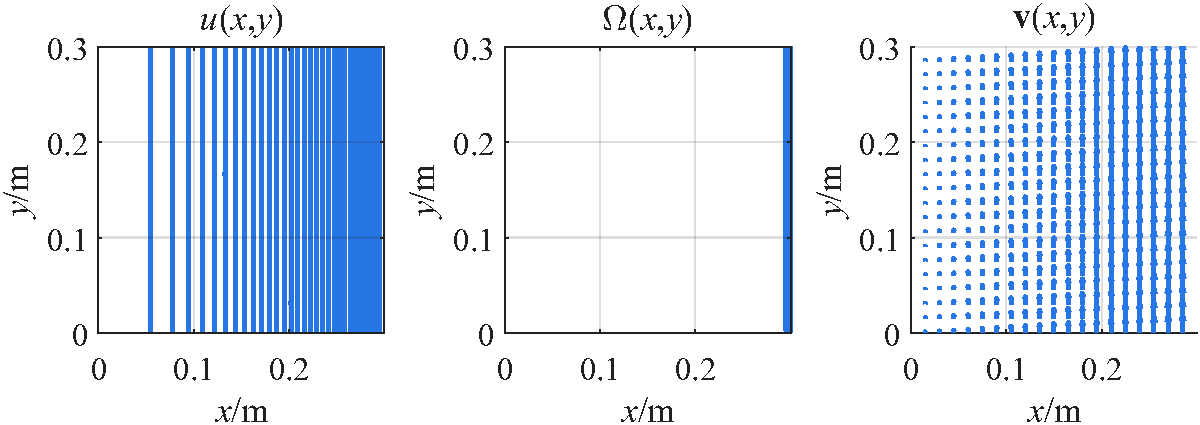
\includegraphics[width=0.8\textwidth]{HaftbWandLinearFelder}
  \caption[Haftbedingung an einer Wand mit linearem Geschwindigkeitsprofil]
  {Haftbedingung an einer Wand. Links haftet das Fluid an einer Wand, rechts
    bewegt es sich mit der Geschwindigkeit $v_0$. Es wird kein Druckgradient
    in $z$-Richtung angenommen. Gezeigt sind Linien f�r konstantes $u(y,z)$
    und konstantes $\Omega(y,z)$ sowie das Geschwindigkeitsfeld.}
  \label{abb:aero_RandDruck0Felder}
\end{figure}
%
Betrachtet man das Geschwindigkeitsprofil (entlang des mittleren Wertes von
$z$) sieht man eindeutig das lineare Geschwindigkeitsprofil in
\figref{aero_RandDruck0Profil}.
%
\begin{figure}[tbp]
  \centering
  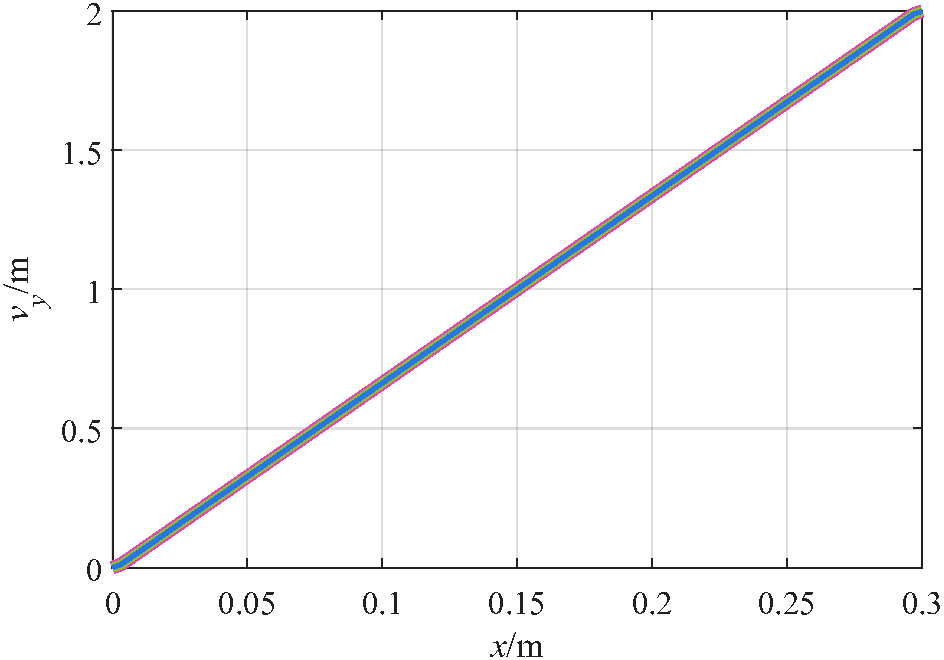
\includegraphics[width=0.5\textwidth]{HaftbWandLinearProfil}
  \caption[Lineares Geschwindigkeitsprofil an einer Wand]
  {Lineares Geschwindigkeitsprofil an einer Wand. Es liegt kein Druckgradient
    vor und $v(y)$ ist f�r den mittleren Wert von $z$ aus
    \figref{aero_RandDruck0Felder} dargestellt.}
  \label{abb:aero_RandDruck0Profil}
\end{figure}
%
F�r den Druckgradienten aus Fall \ref{item:aero_RandDruck1},
\begin{equation*}
  \frac{1}{2\eta} \frac{\partial p(z)}{\partial z} = \frac{v_0}{b^2} \; ,
\end{equation*}
sind $u(y,z)$, $\Omega(y,z)$ und das Geschwindigkeitsfeld in
\figref{aero_RandDruck1Felder} dargestellt.
%
\begin{figure}[tbp]
  \centering
  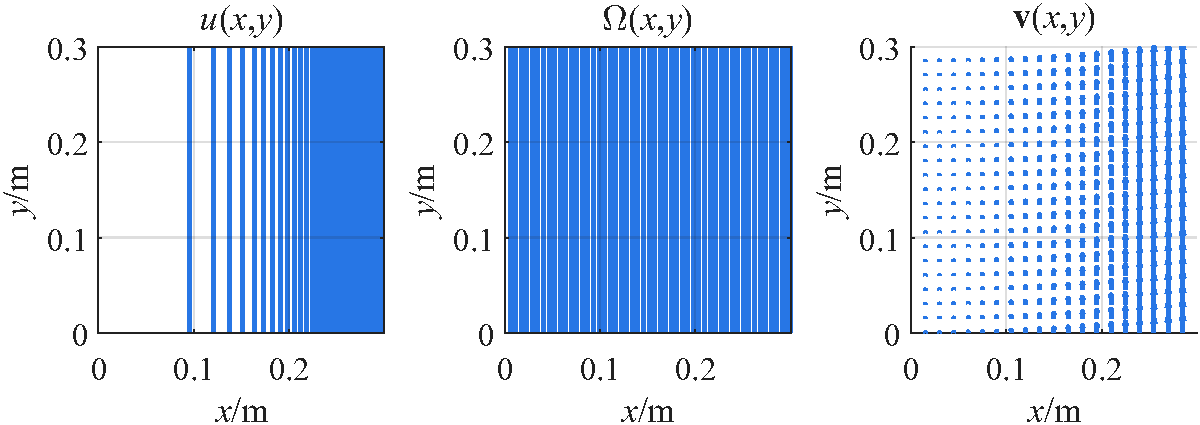
\includegraphics[width=0.8\textwidth]{HaftbWandScheitelLFelder}
  \caption[Haftbedingung an einer Wand mit parabelf�rmigen
  Geschwindigkeitsprofil und Scheitel an der Wand]
  {Haftbedingung an einer Wand. Links haftet das Fluid an einer Wand, rechts
    bewegt es sich mit der Geschwindigkeit $v_0$. Es liegt eine Druckgradient
    von $1/(2\eta)\, \partial p(z)/\partial z = v_0/b^2$ vor. Gezeigt sind
    Linien f�r konstantes $u(y,z)$ und konstantes $\Omega(y,z)$ sowie das
    Geschwindigkeitsfeld.}
  \label{abb:aero_RandDruck1Felder}
\end{figure}
%
In der Darstellung des Geschwindigkeitsprofils in
\figref{aero_RandDruck1Profil} sieht man eindeutig den Scheitel am linken
Rand.
%
\begin{figure}[tbp]
  \centering
  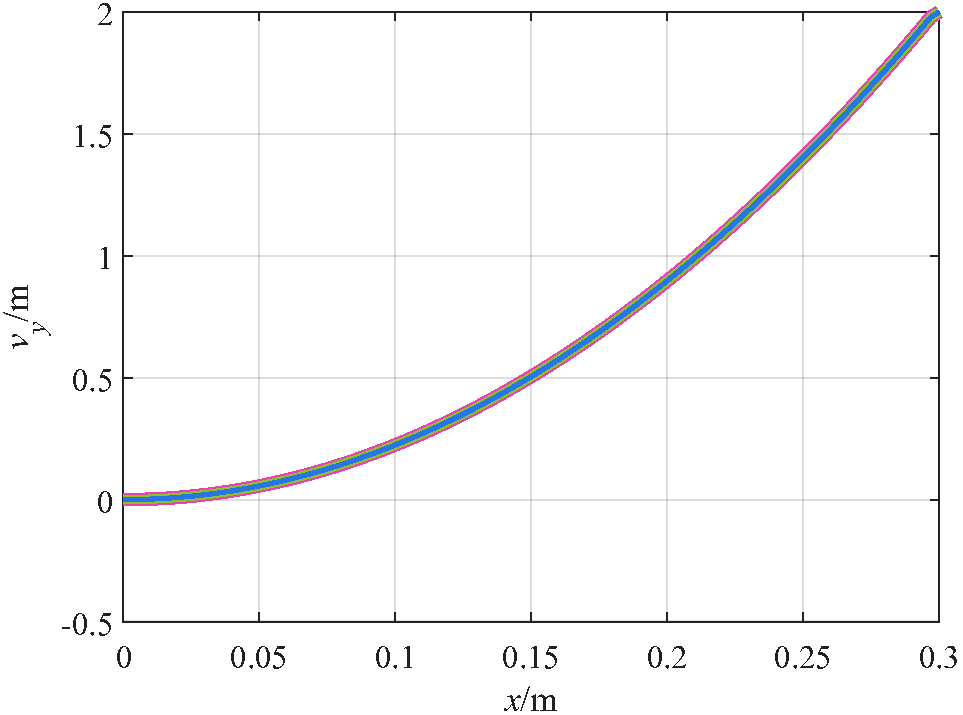
\includegraphics[width=0.5\textwidth]{HaftbWandScheitelLProfil}
  \caption[Parabelf�rmiges Geschwindigkeitsprofil mit Scheitel an der Wand]
  {Parabelf�rmiges Geschwindigkeitsprofil mit Scheitel an der Wand. Es liegt
    ein Druckgradient von $1/(2\eta)\, \partial p(z)/\partial z =
    v_0/b^2$ vor und $v(y)$ ist f�r den mittleren Wert von $z$ aus
    \figref{aero_RandDruck1Felder} dargestellt.}
  \label{abb:aero_RandDruck1Profil}
\end{figure}
%
Vollkommen analog findet man f�r den Druckgradienten aus Fall
\ref{item:aero_RandDruck2},
\begin{equation*}
  \frac{1}{2\eta} \frac{\partial p(z)}{\partial z} = -\frac{v_0}{b^2}  \; ,
\end{equation*}
die Werte $u(y,z)$, $\Omega(y,z)$ und das Geschwindigkeitsfeld aus
\figref{aero_RandDruck2Felder}.
%
\begin{figure}[tbp]
  \centering
  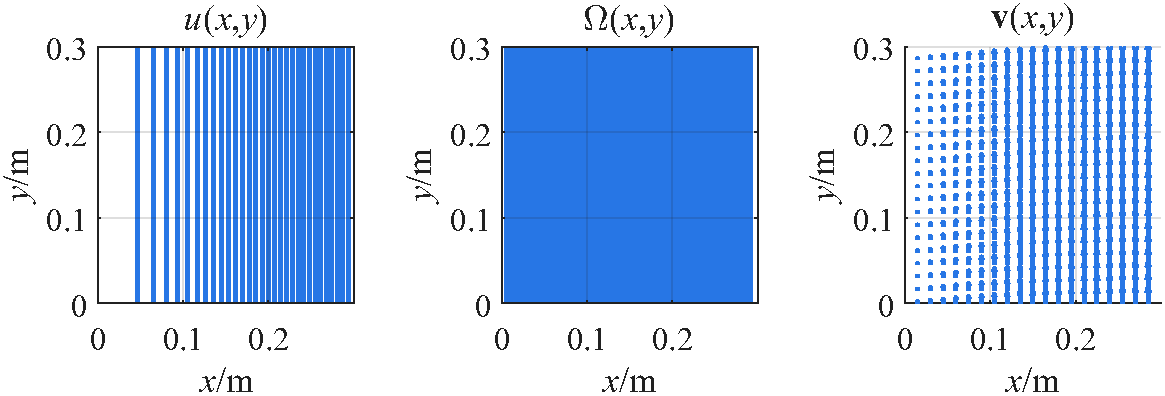
\includegraphics[width=0.8\textwidth]{HaftbWandScheitelRFelder}
  \caption[Haftbedingung an einer Wand mit parabelf�rmigen
  Geschwindigkeitsprofil und Scheitel an der Wand]
  {Haftbedingung an einer Wand. Links haftet das Fluid an einer Wand, rechts
    bewegt es sich mit der Geschwindigkeit $v_0$. Es liegt eine Druckgradient
    von $1/(2\eta)\, \partial p(z)/\partial z = -v_0/b^2$ vor. Gezeigt sind
    Linien f�r konstantes $u(y,z)$ und konstantes $\Omega(y,z)$ sowie das
    Geschwindigkeitsfeld.}
  \label{abb:aero_RandDruck2Felder}
\end{figure}
%
In der Darstellung des Geschwindigkeitsprofils in
\figref{aero_RandDruck1Profil} sieht man eindeutig, dass hier der Scheitel
am rechten Rand liegt, also dort, wo die Geschwindigkeit maximal ist.
%
\begin{figure}[tbp]
  \centering
  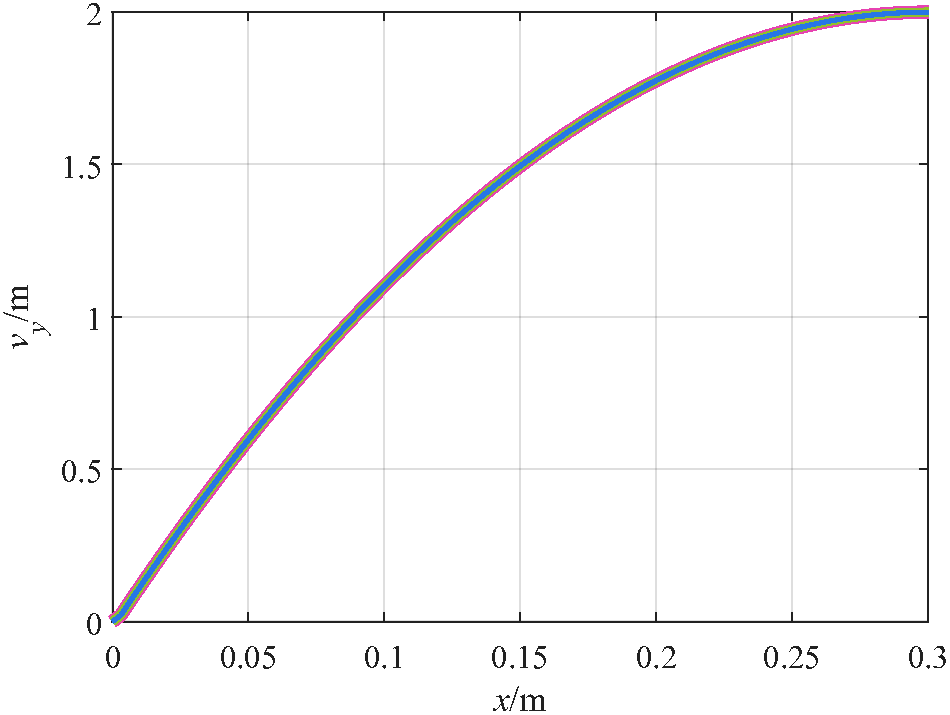
\includegraphics[width=0.5\textwidth]{HaftbWandScheitelRProfil}
  \caption[Parabelf�rmiges Geschwindigkeitsprofil mit Scheitel bei der
  maximalen Geschwindigkeit]
  {Parabelf�rmiges Geschwindigkeitsprofil mit Scheitel bei der maximalen
    Geschwindigkeit. Es liegt ein Druckgradient von $1/(2\eta)\, \partial
    p(z)/\partial z = -v_0/b^2$ vor und $v(y)$ ist f�r den mittleren Wert von
    $z$ aus \figref{aero_RandDruck2Felder} dargestellt.}
  \label{abb:aero_RandDruck2Profil}
\end{figure}
%


\end{sol} 
\textcolor{blue} {$\rightarrow$ zur} \probref{aero_haftwand}.\\
\noindent\rule[1ex]{\textwidth}{0.5pt}  \newpage  



\newpage


\section{\mscre}\label{kap:aero_matlabskripts}

Die mathematisch-physikalische Behandlung von Problem



\clearpage
\setcounter{chapter}{4}
\setcounter{section}{3}
\setcounter{subsection}{0}
\setcounter{figure}{0}
\setcounter{equation}{0}
\setcounter{prob}{0}
\counterwithin{table}{section}
\setcounter{table}{0}
\section{L�sungsbeispiele \autoref{chap:spo} -- Physik des Sports}\label{kap:spo_lsguebungen}

\begin{sol}{prob:spo_energyconsumption}\label{lsg:spo_energyconsumption} %�bung1
\textbf{Absch�tzung Energieverbrauch} \\ 

Text

\end{sol} 
\textcolor{blue} {$\rightarrow$ zur} \probref{spo_energyconsumption}.\\
\noindent\rule[1ex]{\textwidth}{0.5pt}  \newpage  


 
%


\section{\mscre}\label{kap:spo_matlabskripts}

Die mathematisch-physikalische Behandlung von Problem



%\newpage
%\thispagestyle{empty}
%\quad 
%\newpage
%\newpage
\end{PartL}

\renewcommand{\thechapter}{A\,\arabic{chapter}}

\begin{PartA}{Appendix}

\setcounter{chapter}{2}
\setcounter{section}{2}
\setcounter{subsection}{0}
\setcounter{equation}{0}
\counterwithin{table}{section}
\setcounter{table}{0}
\newpage
\thispagestyle{empty}
\quad 
\newpage
\newpage
\section{Formelsammlung zur Aerodynamik}\label{kap:aero_formelsammlung}
Im Folgenden geben wir zum Arbeitsbuch einige h�ufig benutzte Formeln und Beziehungen der Aerodynamik.




\newpage
\section{Formelsammlung zur Sportphysik}\label{kap:spo_formelsammlung}
Im Folgenden geben wir zum Arbeitsbuch einige h�ufig benutzte Formeln und Beziehungen der Sportphysik.


\newpage
\addcontentsline{toc}{chapter}{Quellenangaben}

\begingroup
\let\cleardoublepage\relax
\bibliography{referenzen}
\phantomsection
\addcontentsline{toc}{section}{Stichwortverzeichnis}
\printindex
\phantomsection
\addcontentsline{toc}{section}{Personenverzeichnis}
\printindex[personen]


\cleardoublepage
\phantomsection
\addcontentsline{toc}{chapter}{MATLAB-Skriptverzeichnis}
\thispagestyle{fancy}
\fancyhead[LO]{\nouppercase{\normalsize MATLAB-Skriptverzeichnis}}
\fancyhead[RE]{\nouppercase{\normalsize MATLAB-Skriptverzeichnis}}

\printindex[mfiles]


\endgroup
\newpage
\thispagestyle{empty}
\quad 
\newpage

\end{PartA}

%%%%%%%%%%%%%%%%%%%%%%%%%%%%%%%%%%%%%%%%%%%%%%%%%%%%%%%%%%%\cdot
%\input{footer.tex}
